\newpage

\chapter{Sprint 2: Equipment Monitoring and Inventory}

\cfoot{\thepage}

\parindent=0.5in
\onehalfspacing

\section{Introduction}

Following the successful completion of Sprint 1 which established authentication and site management foundations, we now focus on Sprint 2 titled "Equipment Monitoring and Inventory". This sprint concentrates on the design and implementation of equipment tracking and inventory management modules essential for comprehensive telecommunications network asset management.

The second sprint extends site management capabilities by introducing detailed equipment inventory tracking, enabling network engineers and technicians to monitor all network hardware across telecommunications sites. This includes managing equipment lifecycle, tracking status changes, and maintaining accurate records of installation and warranty information critical for proactive network maintenance.

\section{Sprint Backlog}

During the sprint planning meeting, we discussed with the Scrum Master the tasks required in this sprint, presented in Table 4.1 below.

\begin{table}[H]
\centering
\small
\begin{tabular}{|p{2.5cm}|p{4cm}|p{2.8cm}|c|c|}
\hline
\textbf{Functionality} & \textbf{User Story} & \textbf{Tasks} & \textbf{Complexity} & \textbf{Est.} \\
\hline
Equipment Registration & 
As admin and engineer, I can add new equipment with serial numbers.
& 
Equipment creation
Serial validation
Testing
& 
Med
Hard  
Med
& 
5
5
3 \\
\hline
Status Tracking & 
As technician, engineer, and admin, I can update equipment status.
& 
Status management
Status interfaces
Testing
& 
Med
Easy
Med
& 
4
2
3 \\
\hline
Equipment Inventory & 
As all users, I can view equipment. As admin and engineer, I can edit.
& 
Equipment CRUD
Equipment interfaces
Testing
& 
Med
Med
Hard
& 
5
4
5 \\
\hline
Equipment Statistics & 
As manager, engineer, and admin, I can view equipment statistics.
& 
Statistics calculation
Dashboard cards
Testing
& 
Med
Easy
Med
& 
4
2
3 \\
\hline
\end{tabular}
\caption{Sprint 2 Backlog}
\label{tab:sprint2_backlog}
\end{table}

\section{Class Diagram}

The class diagram for this sprint focuses on equipment management and relationships with telecommunications sites.

\begin{figure}[H]
    \centering
    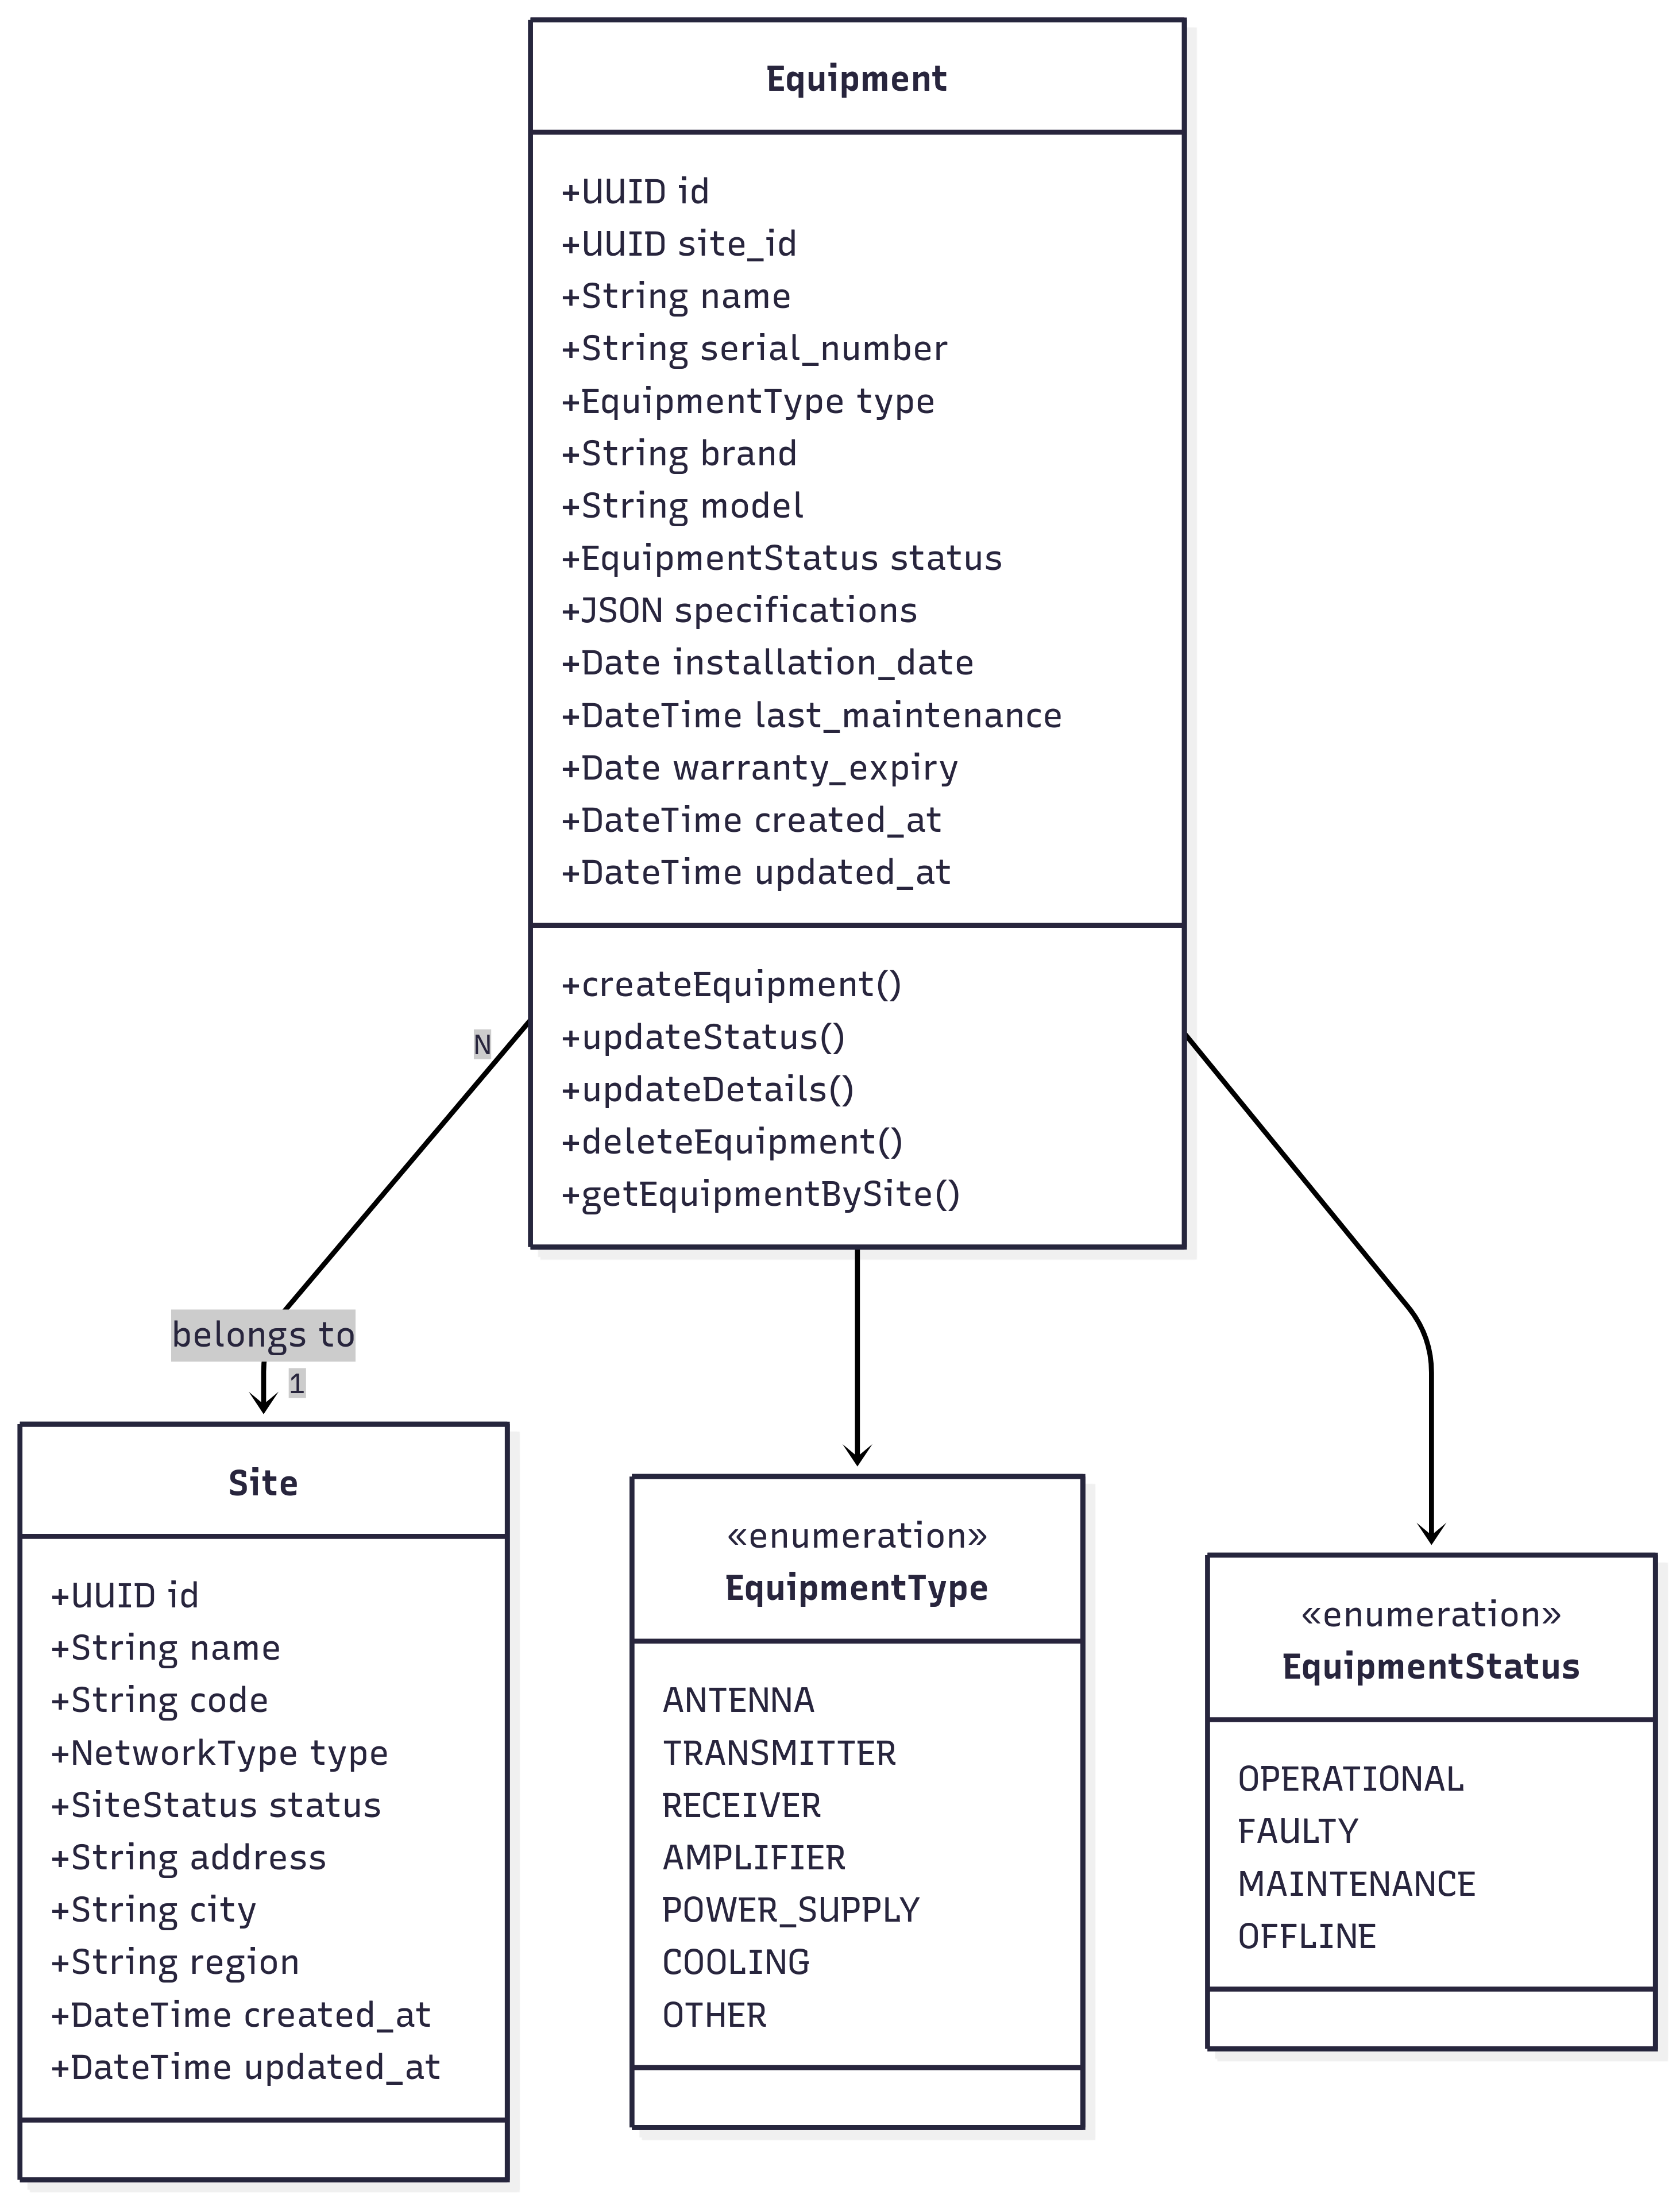
\includegraphics[width=0.8\linewidth]{img/chap_04/equipment_class_diagram.png}
    \caption{Class Diagram "Equipment Monitoring and Inventory"}
    \label{fig:class_diagram_sprint2}
\end{figure}

The diagram illustrates the relationship between \texttt{Equipment} and \texttt{Sites}. The \texttt{Equipment} class maintains unique serial numbers, equipment type classifications, operational status, brand and model information, and warranty details. The \texttt{EquipmentType} and \texttt{EquipmentStatus} enumerations ensure controlled values. The many-to-one relationship ensures every equipment item is associated with a specific network location.

\section{Use Case Diagram}

The use case diagram shows actors and their hierarchical interactions with the equipment management system.

\begin{figure}[H]
    \centering
    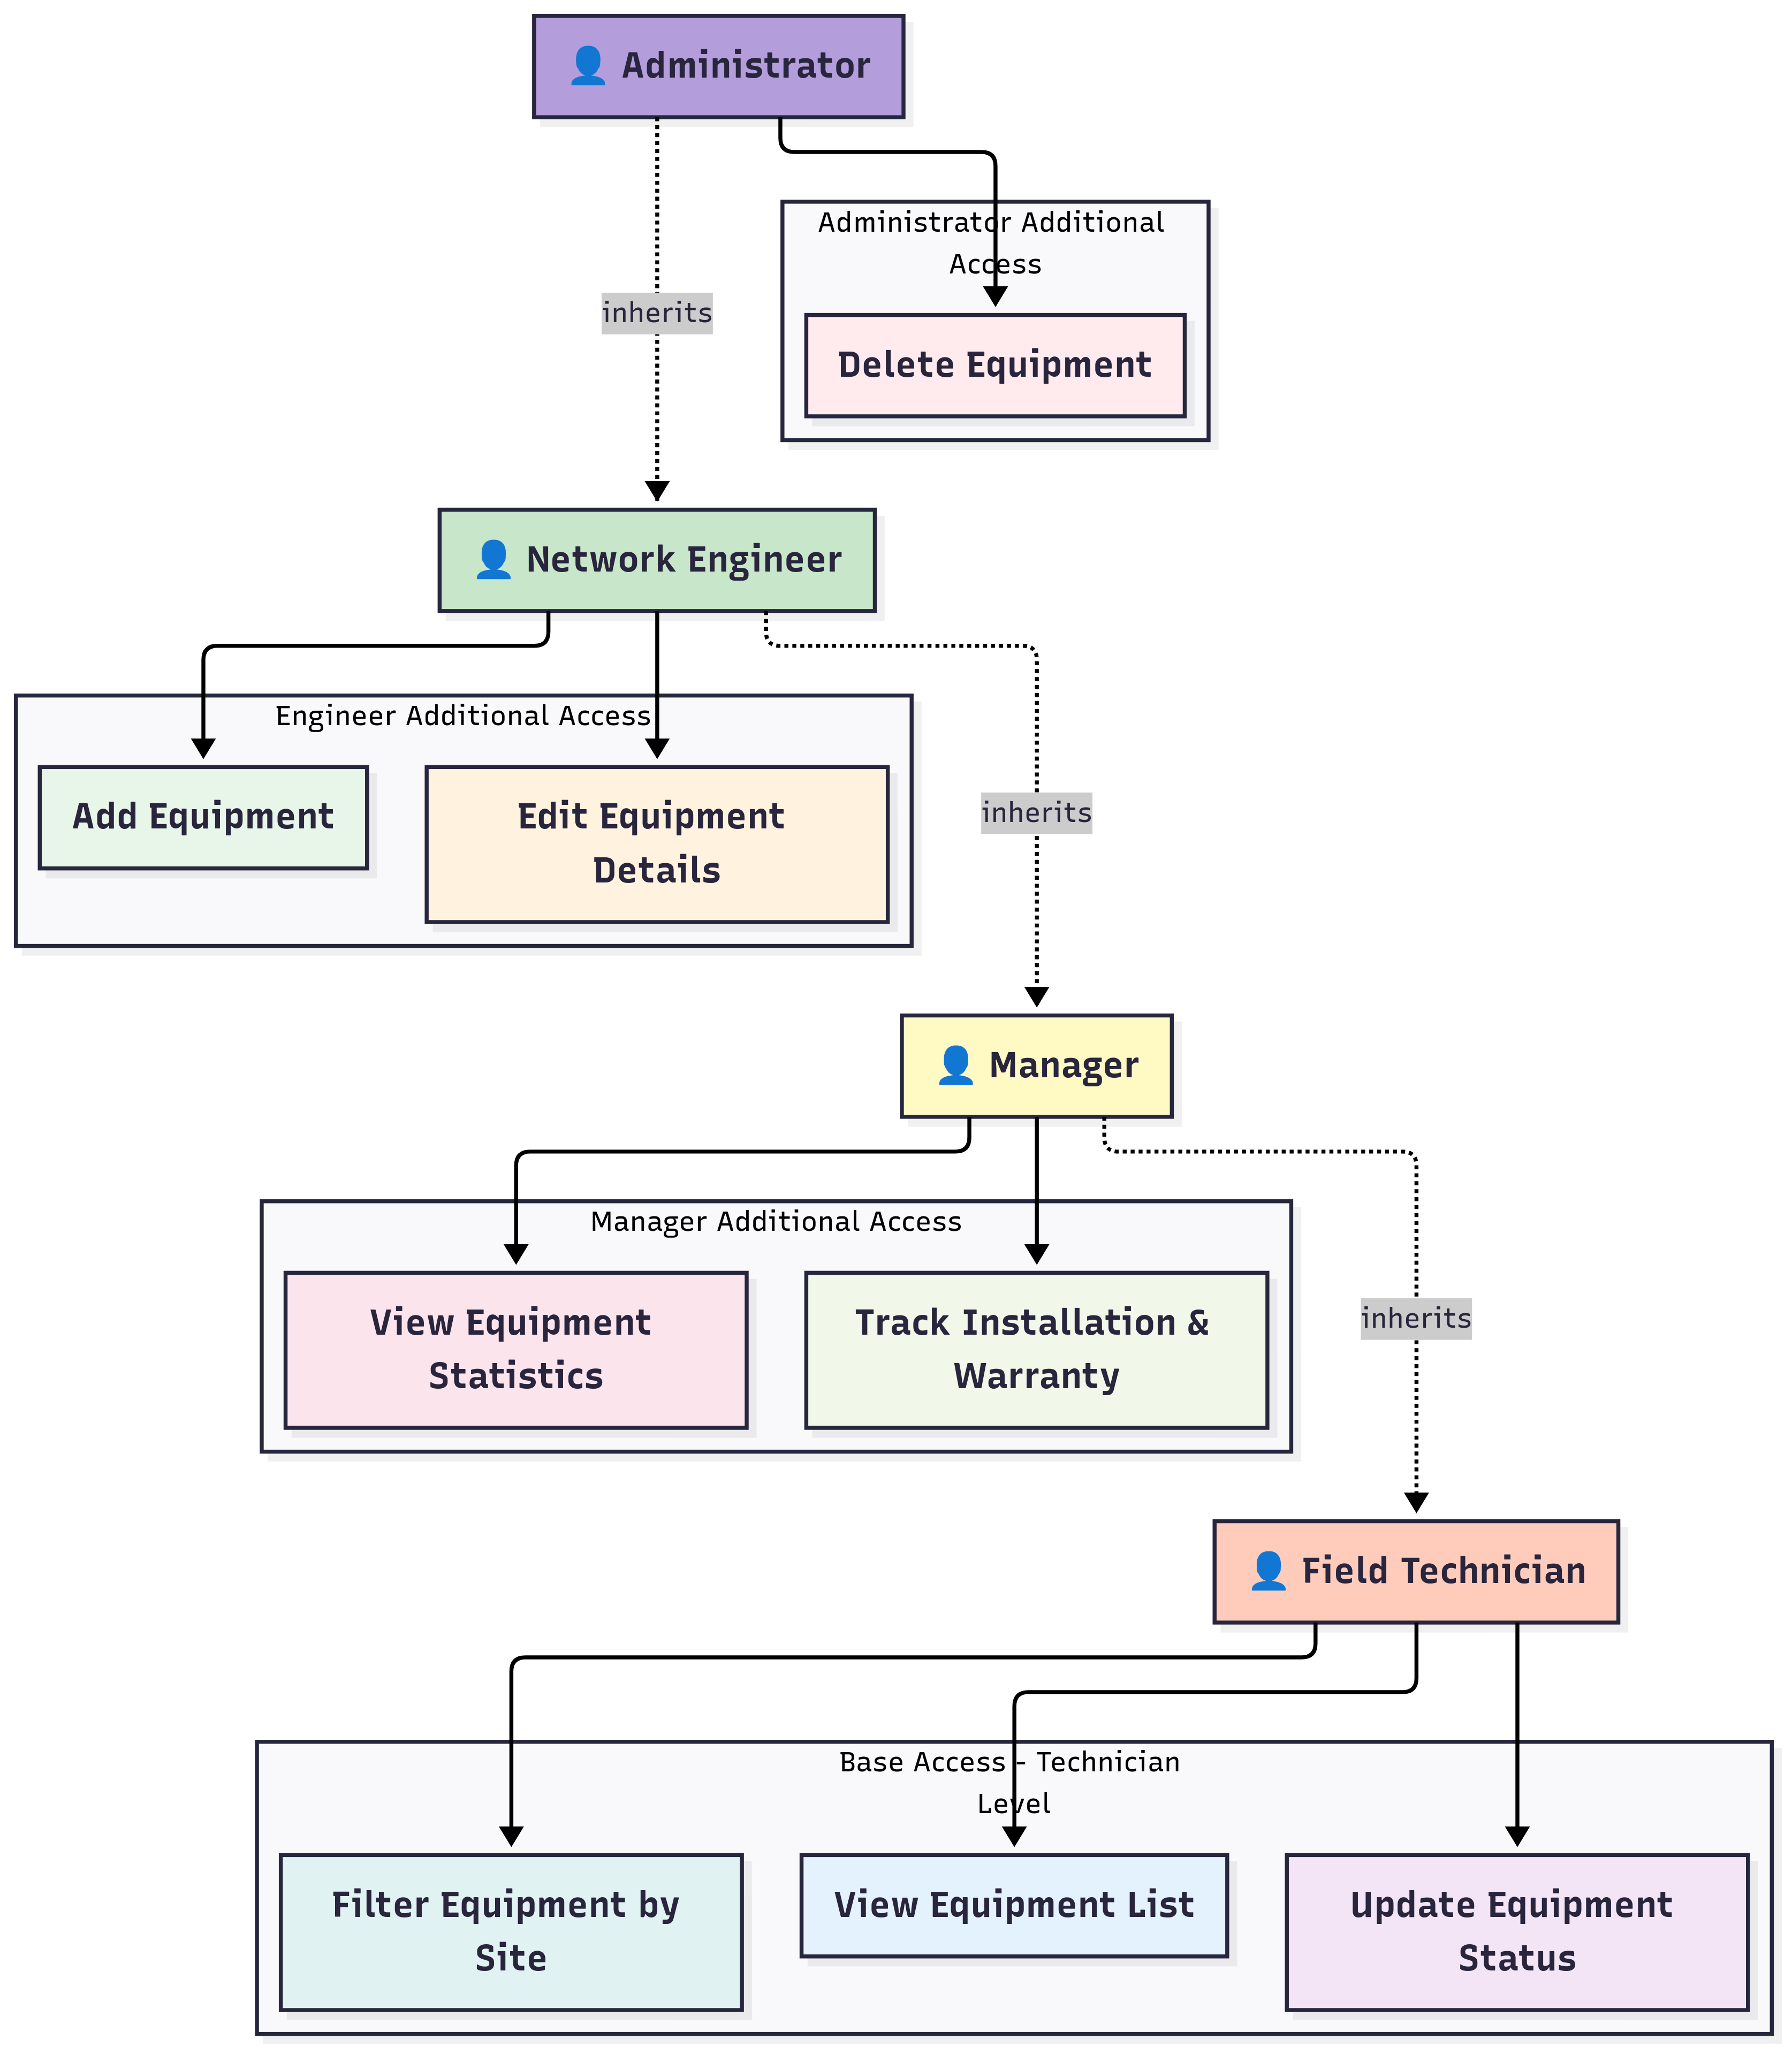
\includegraphics[width=0.75\linewidth]{img/chap_04/equipment_usecase_diagram.png}
    \caption{Use Case Diagram "Equipment Monitoring and Inventory"}
    \label{fig:use_case_diagram_sprint2}
\end{figure}

The diagram implements an inheritance hierarchy across four actor types. Field Technicians have base access (view, update status, filter by site). Managers inherit technician permissions plus statistics and warranty tracking. Network Engineers inherit manager permissions plus add and edit equipment. Administrators inherit all engineer permissions plus exclusive deletion rights.

\begin{table}[H]
\centering
\caption{Equipment Management Permissions by Role}
\label{tab:equipment-permissions}
\small
\begin{tabular}{|p{3.5cm}|c|c|c|c|}
\hline
\textbf{Use Case} & \textbf{Tech} & \textbf{Mgr} & \textbf{Eng} & \textbf{Admin} \\
\hline
View Equipment List & Yes & Yes & Yes & Yes \\
\hline
Update Equipment Status & Yes & Yes & Yes & Yes \\
\hline
Filter Equipment by Site & Yes & Yes & Yes & Yes \\
\hline
View Equipment Statistics & No & Yes & Yes & Yes \\
\hline
Track Installation \& Warranty & No & Yes & Yes & Yes \\
\hline
Add Equipment & No & No & Yes & Yes \\
\hline
Edit Equipment Details & No & No & Yes & Yes \\
\hline
Delete Equipment & No & No & No & Yes \\
\hline
\end{tabular}
\end{table}

Table 4.2 shows the permission matrix. Technicians have three capabilities, managers have five, engineers have seven, and administrators have eight (all capabilities).

\subsection{Use Case Description: Add Equipment}

Table 4.3 provides detailed information on the "Add Equipment" use case.

\begin{table}[H]
\centering
\small
\begin{tabular}{|p{3cm}|p{7.5cm}|}
\hline
\textbf{Use Case} & Add Equipment \\
\hline
\textbf{Primary Actors} & Administrator, Network Engineer \\
\hline
\textbf{Pre-condition} & User authenticated with appropriate role; active site exists \\
\hline
\textbf{Post-condition} & Equipment created in database with operational status \\
\hline
\textbf{Main Scenario} & 
1. User accesses equipment management interface.
2. User clicks "Add Equipment" button.
3. User fills form (name, serial, type, brand, site).
4. User submits form.
5. System validates fields and serial uniqueness.
6. System verifies permissions via RLS.
7. System creates equipment record.
8. System updates equipment list.
\\
\hline
\textbf{Exception Scenarios} & 
Error message if missing data, duplicate serial, invalid type, insufficient permissions, or connection problems.
\\
\hline
\end{tabular}
\caption{Use Case: Add Equipment}
\label{tab:add_equipment_usecase}
\end{table}

\section{Sequence Diagrams}

Sequence diagrams provide detailed explanations of the main processes in this sprint.

\subsection{Add Equipment Sequence Diagram}

\begin{figure}[H]
    \centering
    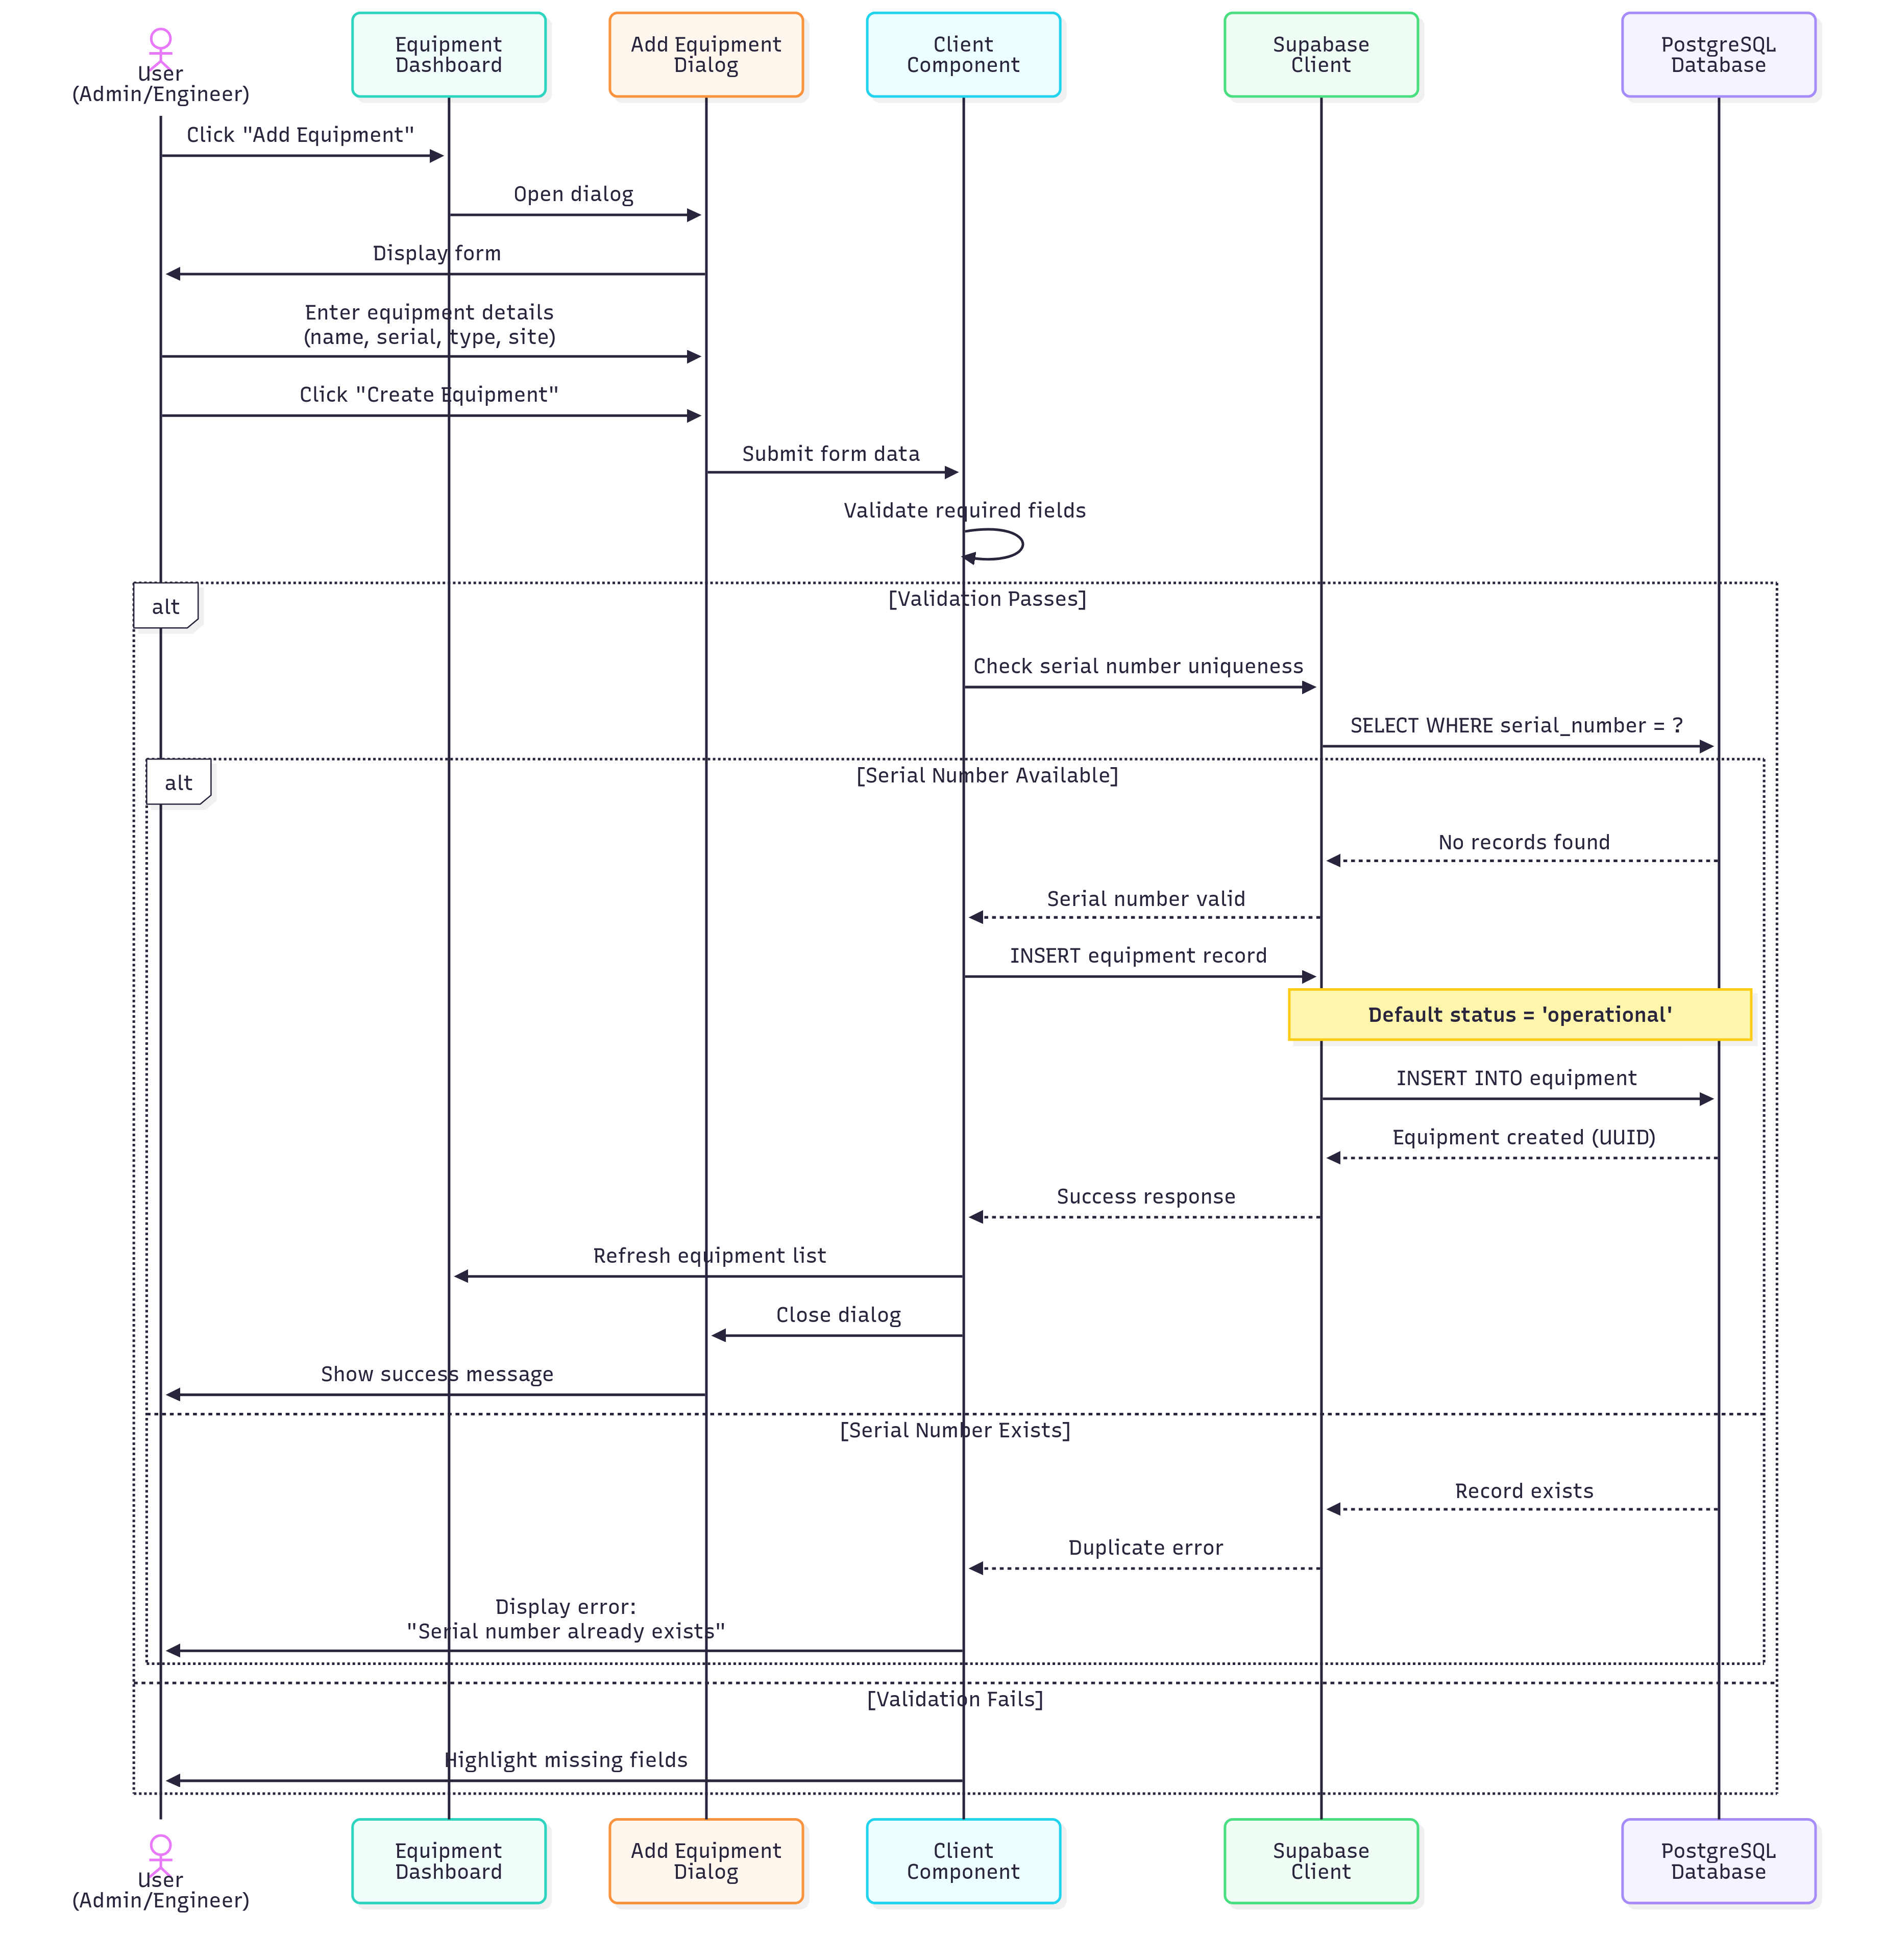
\includegraphics[width=0.85\linewidth]{img/chap_04/add_equipment_sequence.png}
    \caption{Sequence Diagram "Add Equipment"}
    \label{fig:sequence_add_equipment}
\end{figure}

The add equipment sequence diagram demonstrates the workflow for registering new network equipment. An authorized user (Administrator or Engineer) accesses the interface and clicks "Add Equipment", displaying a creation modal. After entering required details (name, serial number, type, site), the user submits the form. The system validates fields and checks serial number uniqueness through database query. If available, the system creates the equipment record with "operational" status via \texttt{supabase.from('equipment').insert()}. Upon success, the equipment list updates in real-time and displays confirmation. Duplicate serial numbers trigger error messages.

\subsection{Edit Equipment Status Sequence Diagram}

\begin{figure}[H]
    \centering
    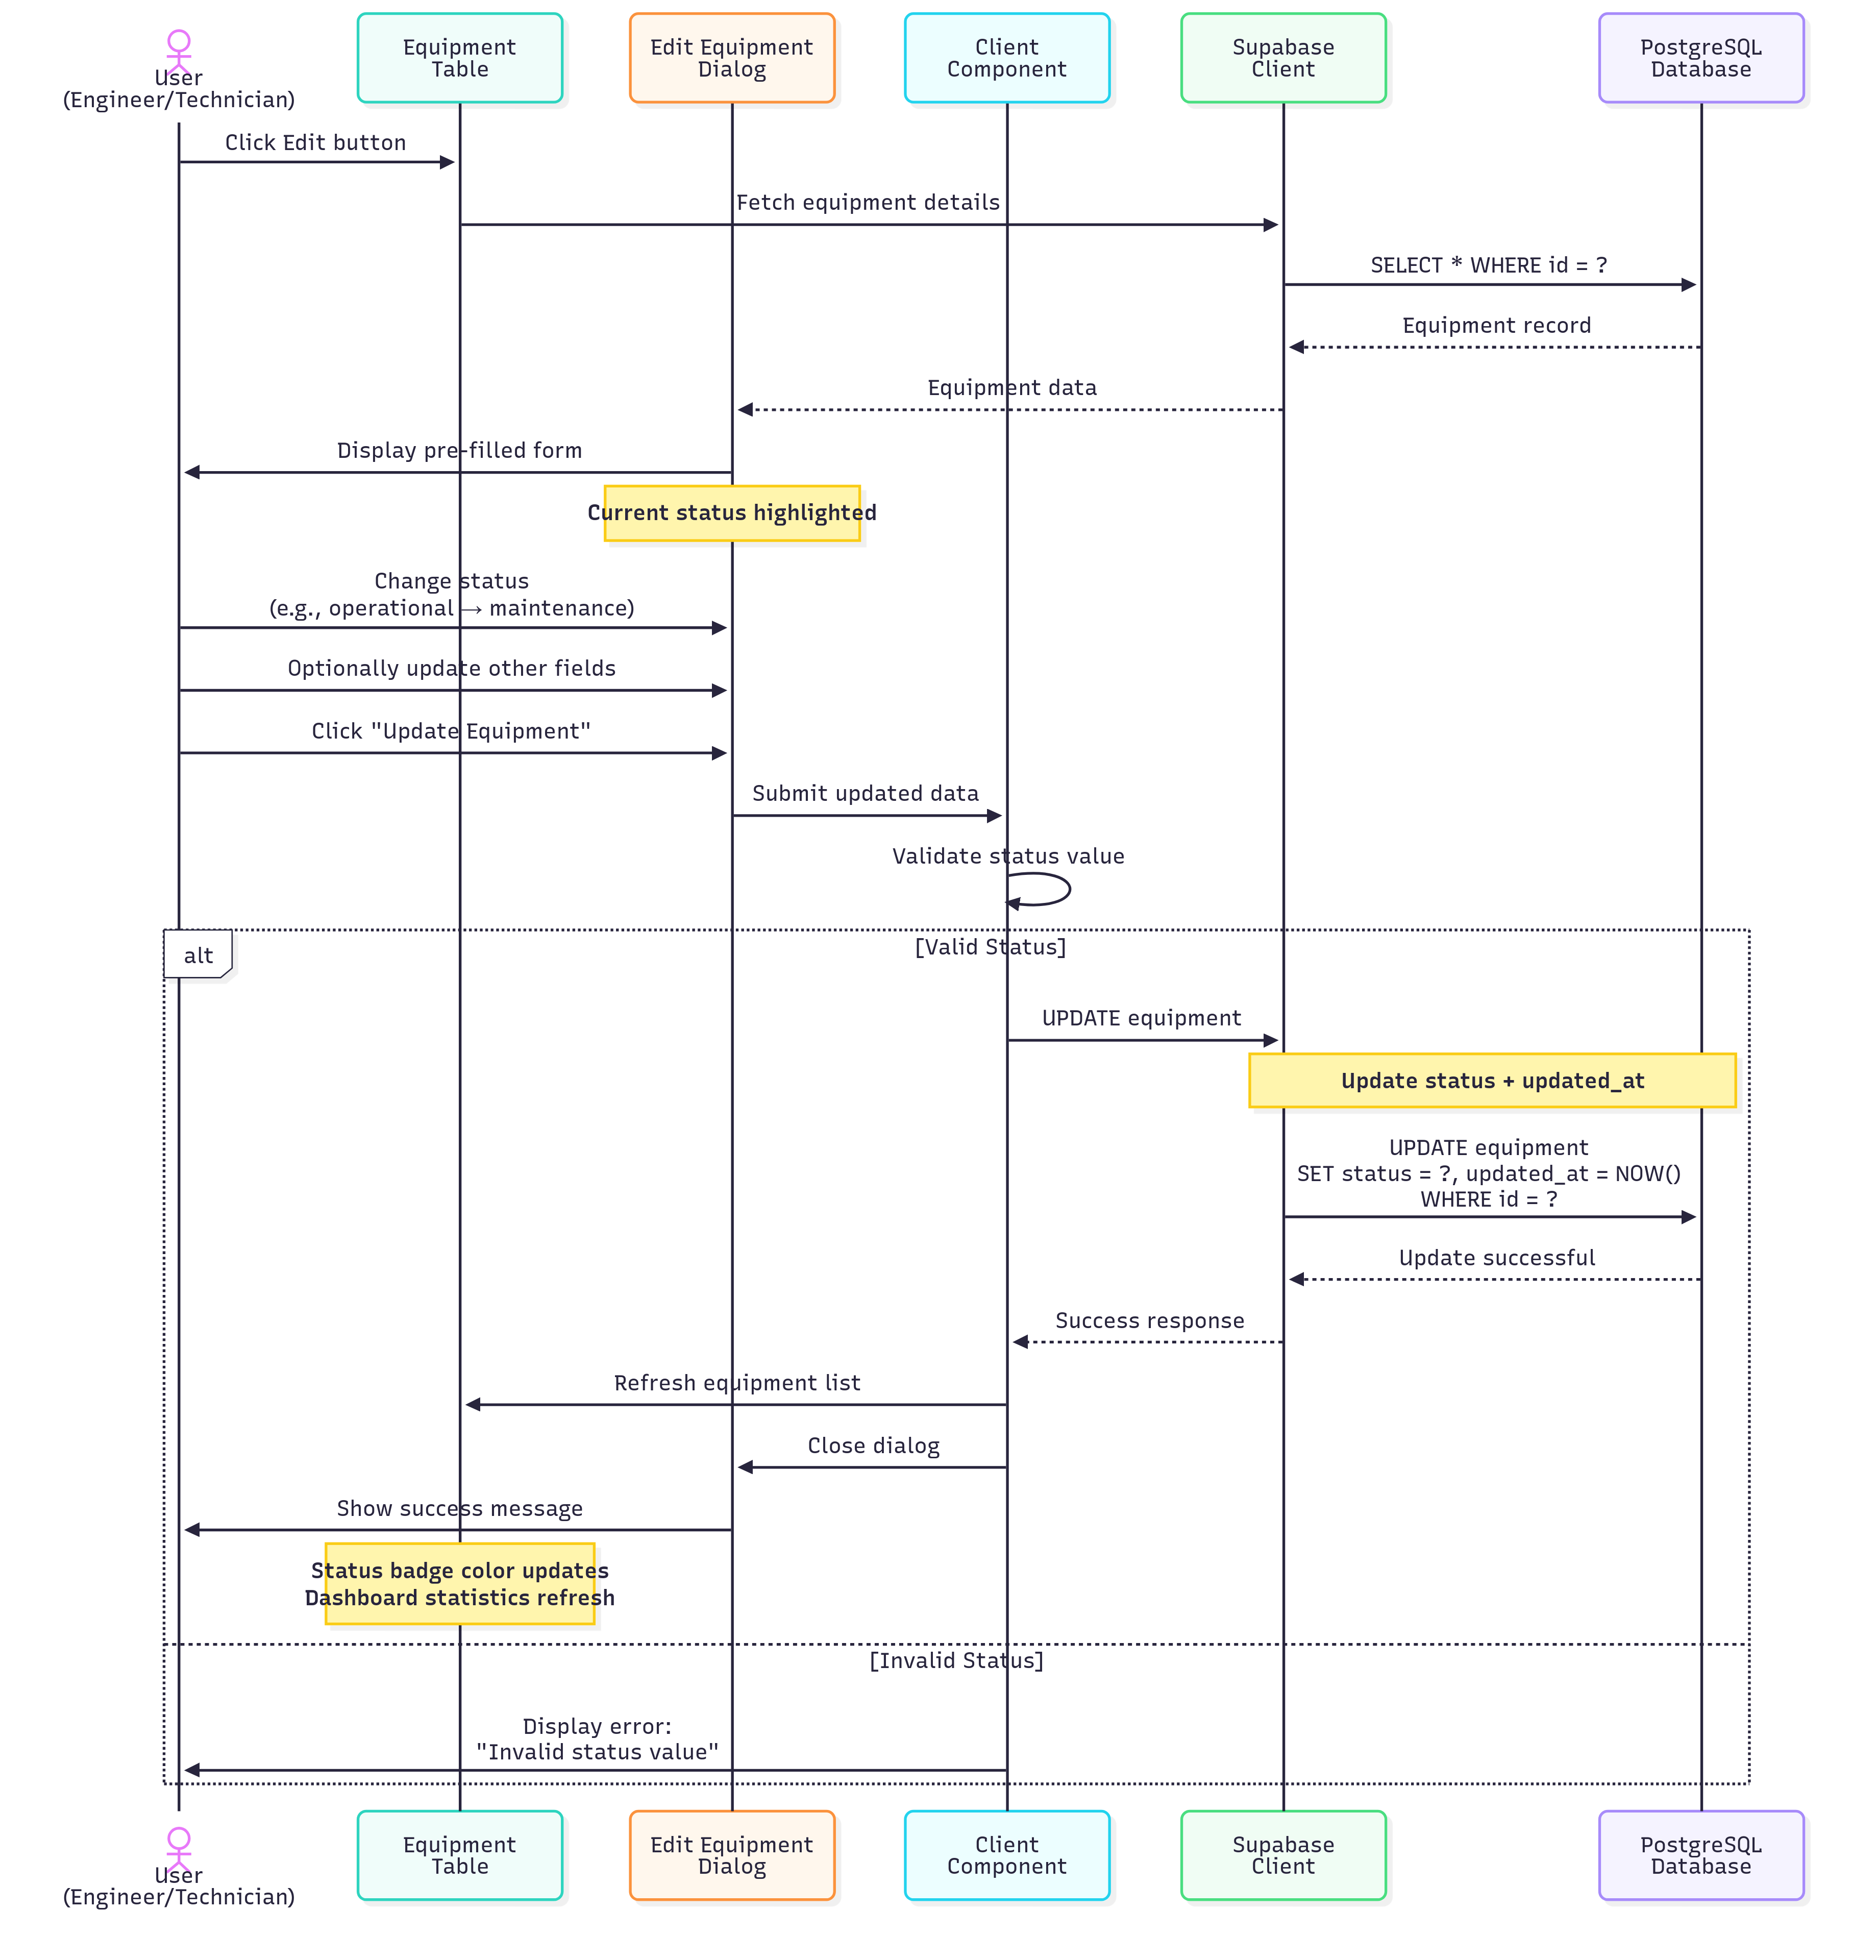
\includegraphics[width=0.85\linewidth]{img/chap_04/edit_equipment_status_sequence.png}
    \caption{Sequence Diagram "Edit Equipment Status"}
    \label{fig:sequence_edit_status}
\end{figure}

The edit status sequence diagram illustrates updating equipment operational state. When a user selects equipment and clicks edit, the system fetches current details including status. The dialog displays pre-filled fields with highlighted current status. The user modifies status (operational, faulty, maintenance, offline) and submits changes. The system validates the status value and sends an UPDATE request. The database verifies permissions through RLS and updates both status and \texttt{updated\_at} timestamp. Upon success, the equipment table refreshes across all sessions, the modal closes, and dashboard statistics recalculate automatically.

\section{Implementation}

Screenshots illustrating the interfaces developed during this sprint.

\subsection{Equipment Dashboard Interface}

\begin{figure}[H]
    \centering
    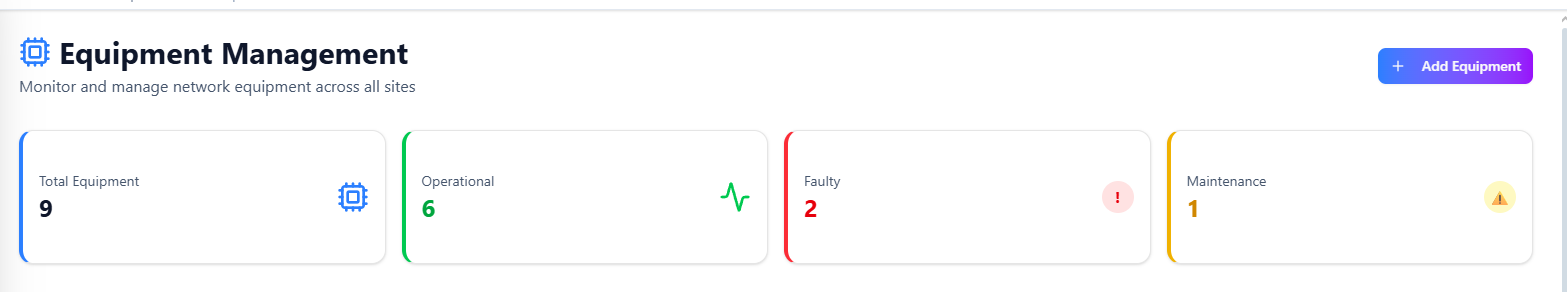
\includegraphics[width=0.8\linewidth]{img/chap_04/equipment_dashboard.png}
    \caption{Equipment Dashboard with Statistics}
    \label{fig:equipment_dashboard}
\end{figure}

The dashboard presents four statistical cards displaying real-time equipment counts by status with color-coded indicators (green: operational, red: faulty, yellow: maintenance, gray: offline).

\subsection{Equipment Management Interface}

\begin{figure}[H]
    \centering
    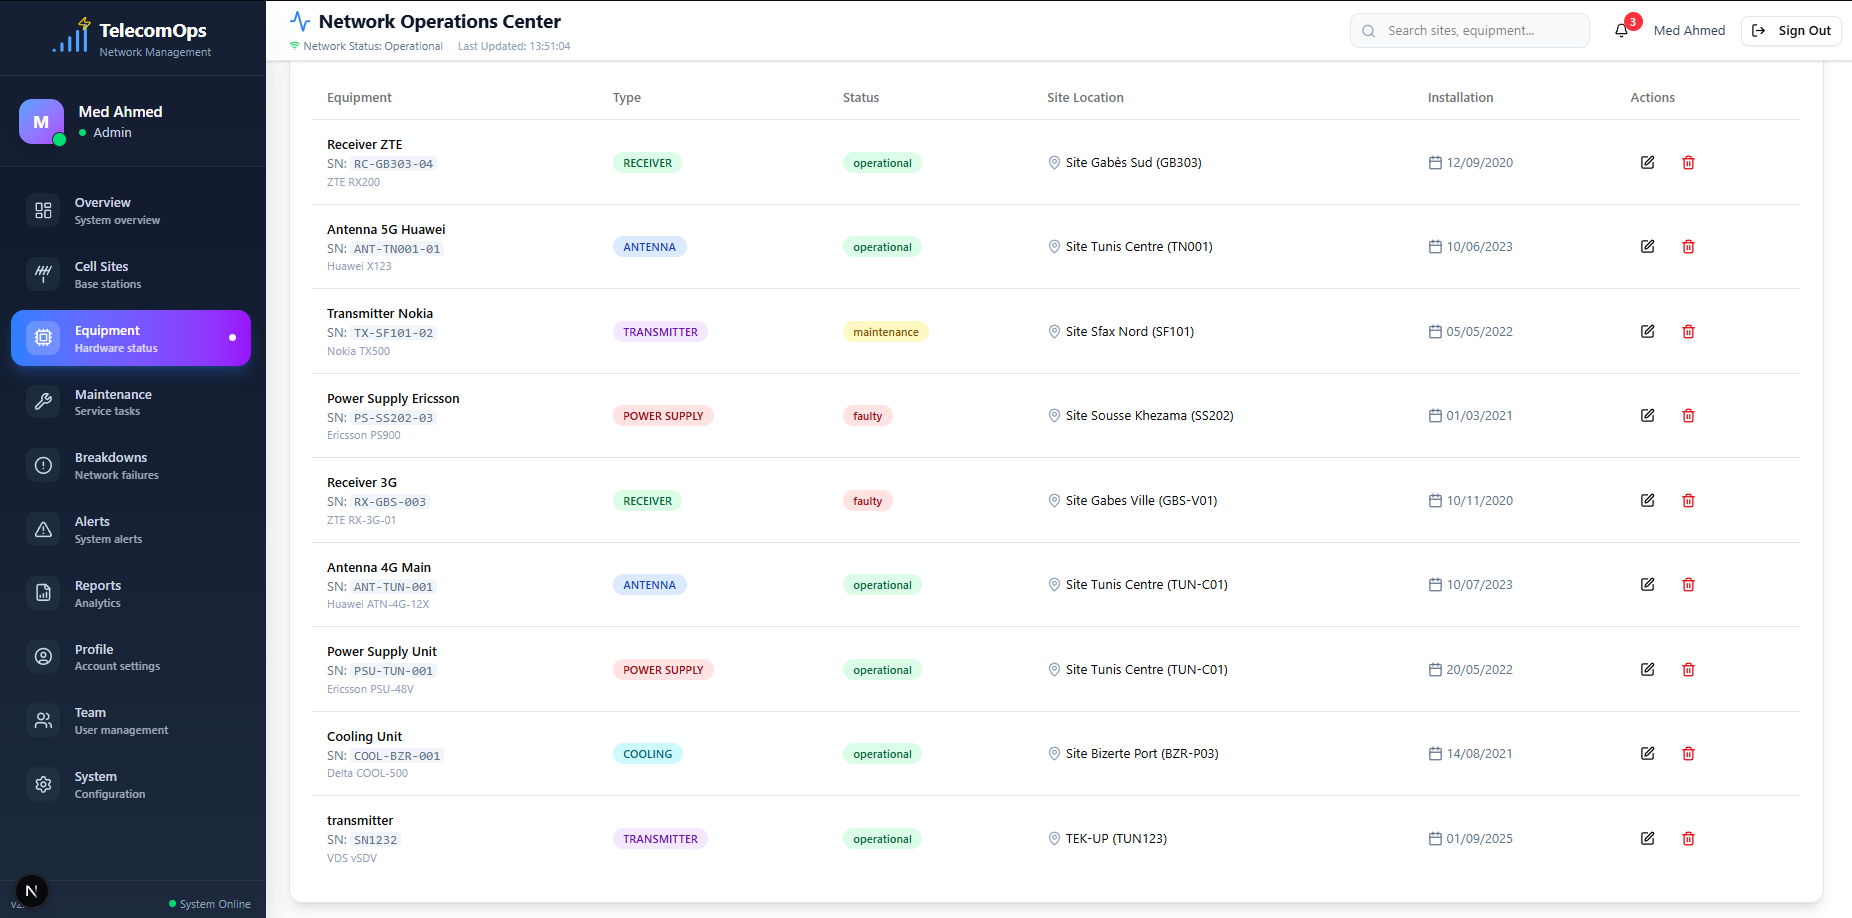
\includegraphics[width=0.8\linewidth]{img/chap_04/equipment_table.png}
    \caption{Equipment Inventory Table}
    \label{fig:equipment_table}
\end{figure}

The equipment table displays comprehensive information with columns for equipment name, serial number, type badge, status badge, site location, installation date, and action buttons.

\subsection{Equipment Management Modals}

\begin{figure}[H]
    \centering
    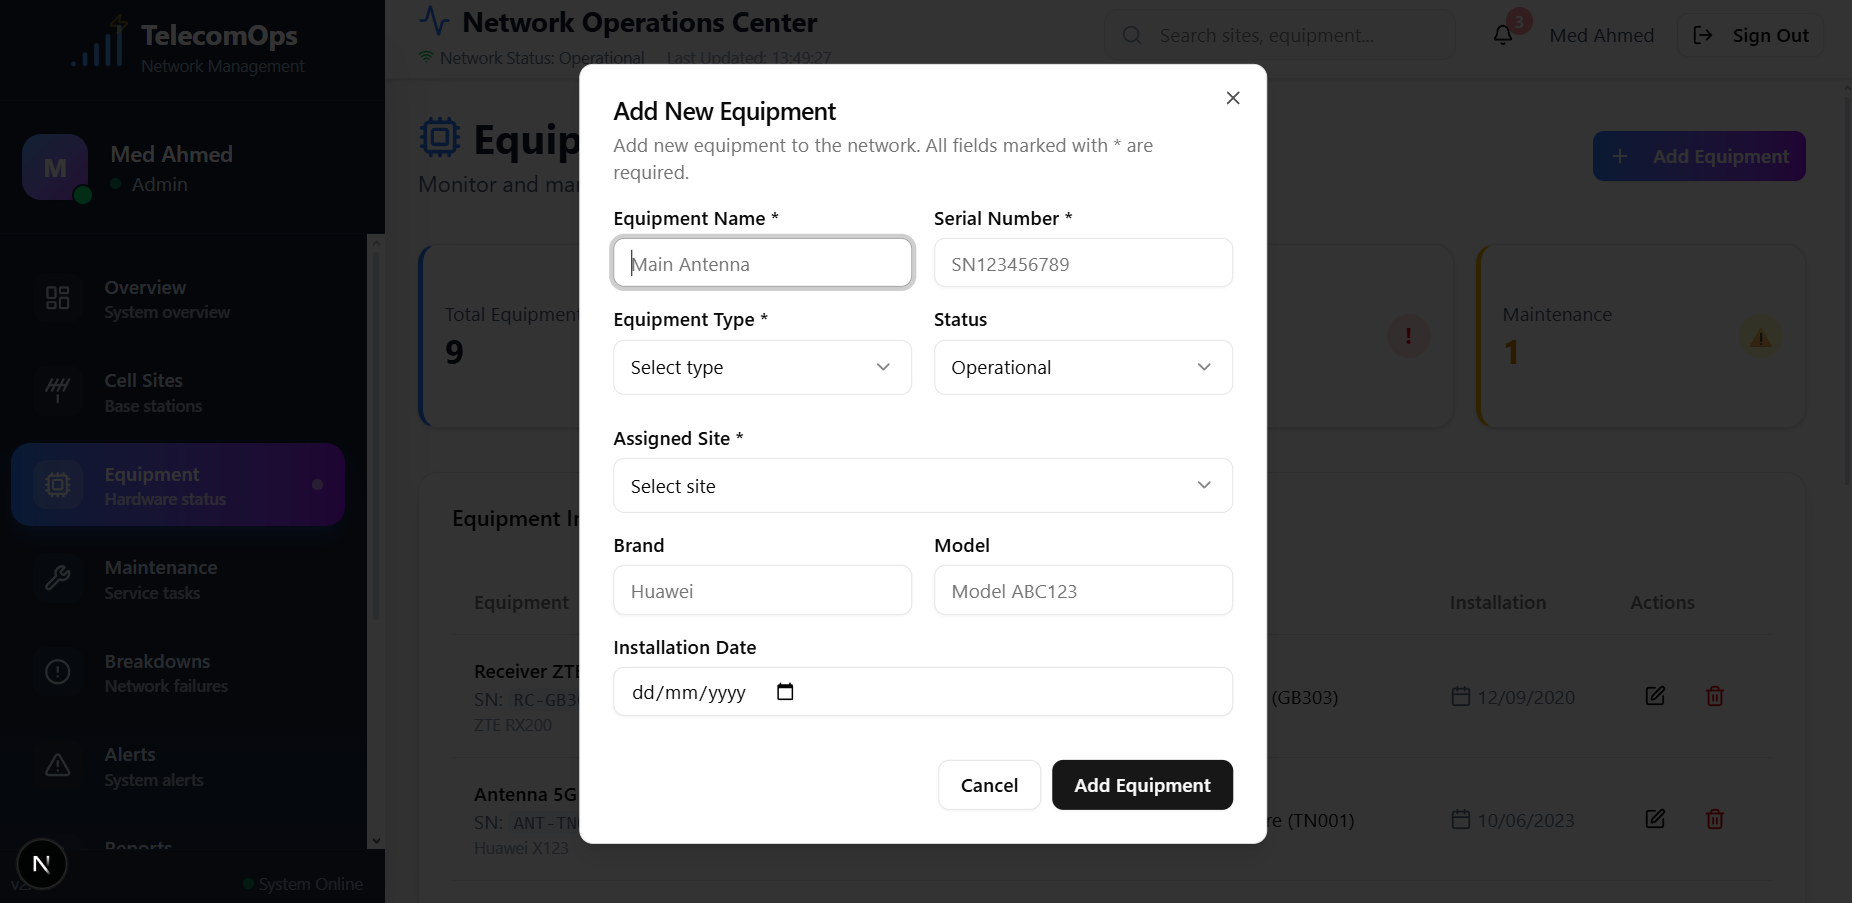
\includegraphics[width=0.6\linewidth]{img/chap_04/add_equipment_dialog.png}
    \caption{Add Equipment Modal}
    \label{fig:add_equipment_modal}
\end{figure}

The add equipment dialog implements required fields (name, serial, type, site) and optional fields (brand, model, installation date).

\begin{figure}[H]
    \centering
    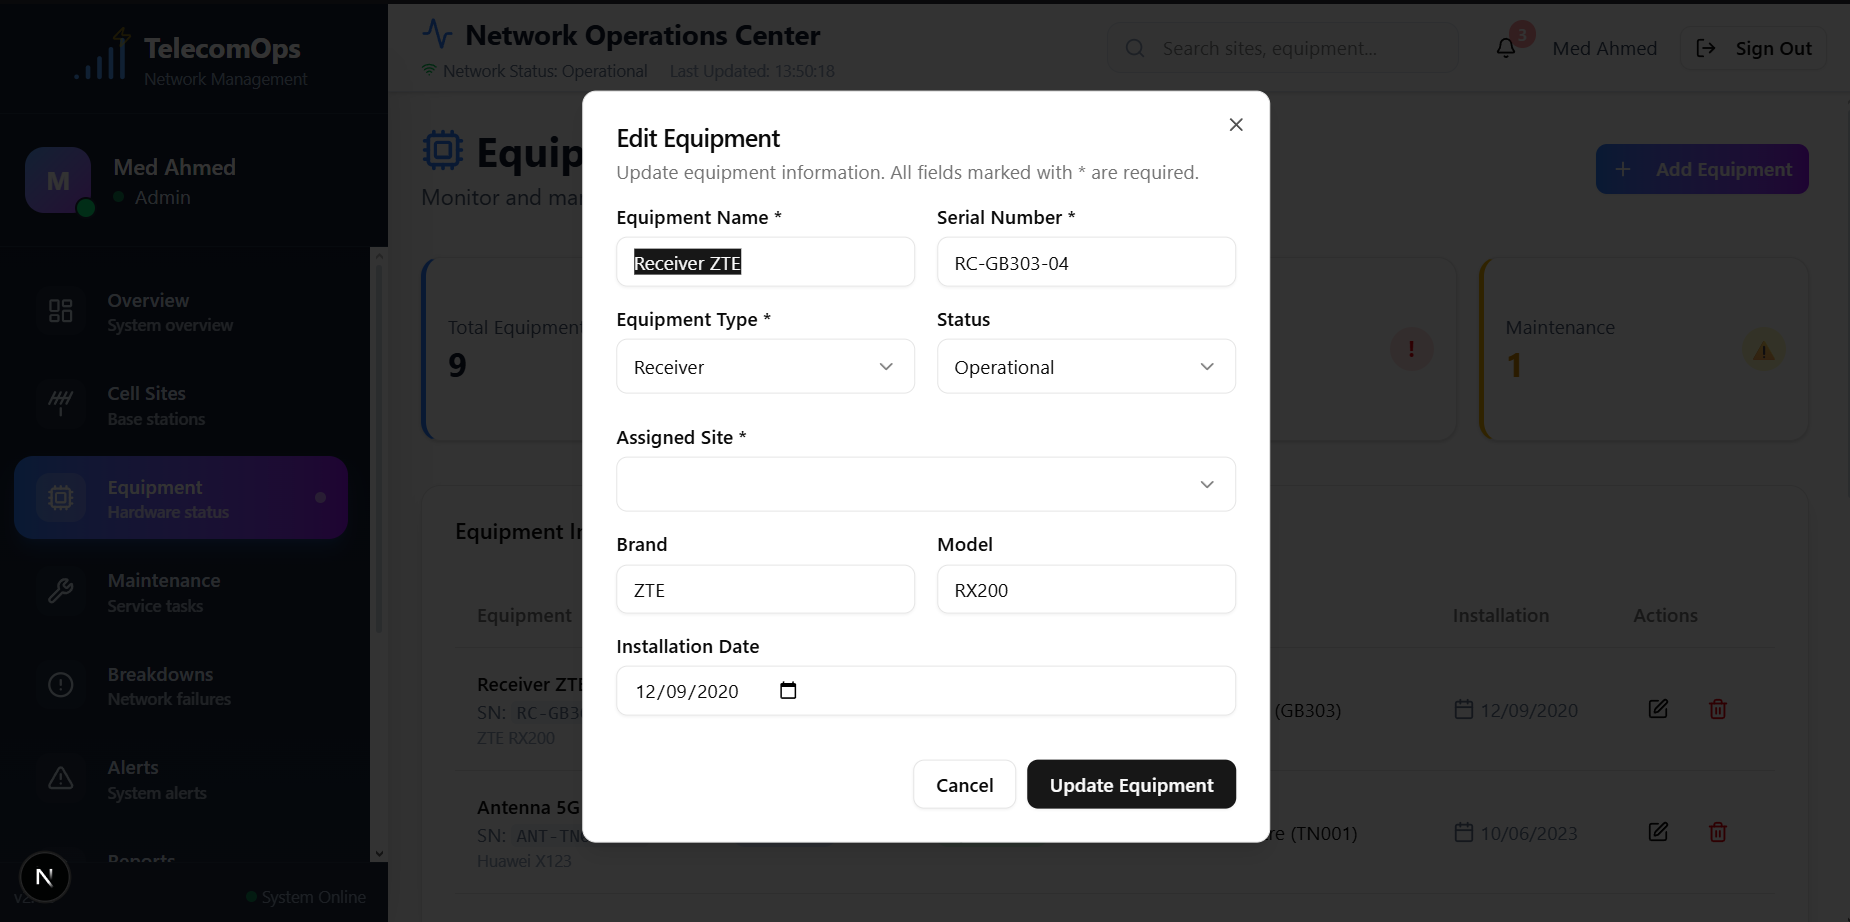
\includegraphics[width=0.6\linewidth]{img/chap_04/edit_equipment_dialog.png}
    \caption{Edit Equipment Modal}
    \label{fig:edit_equipment_modal}
\end{figure}

The edit dialog pre-populates with current information. Serial number remains immutable for traceability.

\section{Technical Challenges and Solutions}

\subsection{Serial Number Uniqueness Validation}

We implemented two-tier validation: client-side format validation for immediate feedback and server-side database queries with unique constraints for absolute enforcement. The equipment table's unique constraint provides database-level protection against duplicates.

\subsection{Equipment Status Management}

We implemented database CHECK constraints defining valid status values (operational, faulty, maintenance, offline) with automatic timestamp updates on \texttt{updated\_at} column, ensuring data integrity while maintaining complete state change history.

\subsection{Site-Equipment Relationship Integrity}

We implemented foreign key relationship with CASCADE deletion policy. The system displays warnings before site deletion showing affected equipment count. NOT NULL constraint on \texttt{site\_id} ensures every equipment maintains valid site association.

\section{Testing and Validation}

\subsection{Equipment CRUD Operations Testing}
Tests confirmed administrators perform all operations, engineers create and update but not delete, technicians view and update status only, and managers have read-only access with statistics.

\subsection{Serial Number Validation Testing}
Extensive testing ensured duplicate prevention. Concurrent creation attempts with identical serial numbers were successfully prevented by database constraints.

\subsection{Equipment Status Transition Testing}
Tests verified status changes update timestamps appropriately, invalid values are rejected, and modifications respect the role-based permission hierarchy.

\section{Conclusion}

This chapter described Sprint 2 focusing on equipment monitoring and inventory management. We performed comprehensive analysis using UML diagrams including class diagrams, use cases with inheritance hierarchy, and sequence diagrams. The implementation delivered complete equipment tracking with role-based access control and real-time status monitoring.

Sprint 2 extended Sprint 1 capabilities by introducing comprehensive equipment inventory management with serial number tracking, status monitoring, and warranty information. The hierarchical role-based permission system ensures logical permission escalation while maintaining security boundaries.

The equipment management system demonstrates effective integration of modern web technologies addressing telecommunications asset management requirements. Quality metrics exceeded targets with successful user acceptance testing across all four roles, establishing robust equipment tracking for network operations.